\documentclass[a4paper,11pt]{article}
\usepackage[utf8]{inputenc}
\usepackage[russian]{babel}
\usepackage[T1]{fontenc}
\usepackage{amssymb,amsmath,clrscode,graphicx,indentfirst}

\author{Иван Веселов}
\title{Курс kiev-clrs -- Лекция 13. Амортизационный анализ}
\date{2009 г.}

\begin{document}

\maketitle
\tableofcontents
\newpage

\setlength{\parskip}{1ex plus 0.5ex minus 0.2ex}

\section{План лекции}
\begin{itemize}
\item Динамические таблицы
\item Групповой анализ
\item Метод бухгалтерского учёта
\item Метод потенциалов
\end{itemize}

\section{Динамические таблицы}

Вопрос: насколько большой должна быть хэш-таблица?
\begin{itemize}
\item нам нужно сделать её как можно больше, т.к. с ростом размера таблицы
  уменьшается время поиска
\item нам нужно сделать её как можно меньше, т.к. в противном случае мы тратим
  много памяти на хранение таблицы
\item Должны соблюдать баланс! $\Theta(n)$ для $n$ ключей.
\end{itemize}

Задача: Но что делать если мы не знаем $n$ наперёд?

Решение: использовать динамические таблицы!

Идея: когда таблица ``переполняется'' (в ней становится слишком много элементов)
-- мы увеличиваем её размер:

\begin{enumerate}
\item выделяем (malloc или new) место для большей таблицы
\item перемещаем элементы из старой таблицы в новую
\item освобождаем память, занимаемую старой таблицей
\end{enumerate}

\begin{figure}[ht]
  \centering
  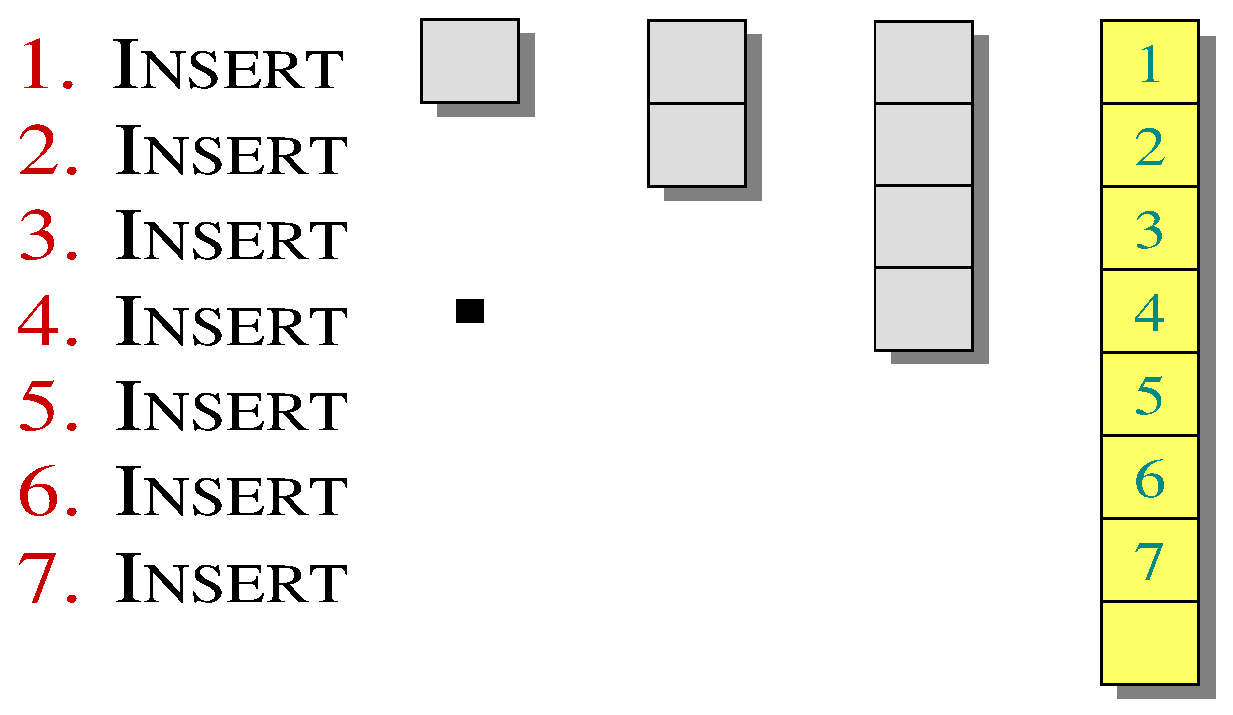
\includegraphics[width=3in]{lecture13/insertion.eps}
  \caption{Пример заполнения динамической таблицы}
  \label{fig:insertion}
\end{figure}


\subsection{Анализ наихудшего случая}
Последовательность из $n$ операций.

Каждая операция выполняется максимум за время $O(n)$.

Значит вся последовательность выполняется за $O(n^2)$?

Анализ неверен! На самом деле последовательность из $n$ операций выполняется за
время $O(n) << O(n^2)$. 

Покажем почему. Пусть $c_i$ -- стоимость $i$-й операции.
$$
c_i = 
\begin{cases}
  i, \text{ если } i - 1 \text{ -- степень двойки}\\
  1, \text{ в противном случае}
\end{cases}
$$



\begin{tabular}{|r|c|c|c|c|c|c|c|c|c|c|}
  \hline
     $i$ & 1 & 2 & 3 & 4 & 5 & 6 & 7 & 8 & 9  & 10 \\
  \hline
$size_i$ & 1 & 2 & 4 & 4 & 8 & 8 & 8 & 8 & 16 & 16 \\
  \hline
   $c_i$ & 1 & 2 & 3 & 1 & 5 & 1 & 1 & 1 & 9  & 1 \\
  \hline
   $c_i$ & 1 & 1 & 1 & 1 & 1 & 1 & 1 & 1 & 1 & 1 \\
         & 0 & 1 & 2 & 0 & 4 & 0 & 0 & 0 & 8 & 1 \\
  \hline
\end{tabular}

Стоимость $n$ операций равна:
$$
\sum_{i=1}^n c_i = n + \sum_{j=0}^{\lfloor \lg(n - 1) \rfloor} 2^j \leqslant n +
2n = 3n = \Theta(n)
$$

Таким образом среднее время выполнения одной операции $\Theta(n) / n =
\Theta(1)$, а не $\Theta(n)$.

Несмотря на то, что некоторые из операций могут быть трудоёмкими, их немного и
их стоимость распределяется по остальным, менее трудоёмким операциям, таким
образом образую хорошую среднюю оценку времени выполнения.

При \emph{амортизационном анализе} время, требуемое для вполнения
последовательности операций над структурой данных, усредняется по \emph{всем}
выполняемым операциям. Этот анализ можно использовать, например, чтобы показать,
что даже если одна из операций является дорогостоящей, то при усреднении по всей
последовательности средняя стоимость операций будет небольшой. Амортизационный
анализ отличается от анализа средних величин тем, что в нём не учитывается
вероятность. При амортизационном анализе гарантируется \emph{средняя
производительность операций в наихудшем случае}.

Три метода проведения амортизационного анализа:

\begin{itemize}
\item групповой анализ (aggregate analysis)
\item метод бухгалтерского учёта (accounting method)
\item метод потенциалов (potential method)
\end{itemize}

Групповой анализ мы только что увидели. В процессе группового анализа
показывается, что в наихудшем случае времия выполнения $n$ операций равно $T(n)$.
Поэтому средняя амортизированная стоимость одной операции равна $T(n)/n$. Этот
метод прост, однако уступает другим методам в точности, поскольку не делает
различия между операциями, присваивая всем операциям (даже разнотипным) равную
амортизированную стоимость.

\section{Метод бухгалтерского учёта}

В этом методе разные по типу операции оцениваются различной стоимостью в
зависимости от фактической стоимости. Величина, которая начисляется на операцию
$i$ называется амортизированной стоимостью $\hat{c}_i$. Если начисленная
стоимость превышает фактическую, то остаток рассматривается как ``кредит'' и
присваивается определённым элементам структуры данных. Кредит может в дальнейшем
использоваться для погашения стоимости более дорогостоящих операций, для оплаты
которых не хватает начисляемой амортизированной стоимости.

Рассмотрим общую схему метода:

\begin{itemize}
\item наделить каждую операцию определённой амортизационной стоимостью
  $\hat{c}_i$. Пускай 1 гр. будет платой за определённую единицу работы.
\item при выполнении операции мы тратим её фактическую стоимость $c_i$
\item не потраченный остаток может быть сохранён в банке (в элементе структуры
  данных) для дальнейшего использования
\item общий баланс должен оставаться положительным, т.е.
$$ \forall{n}: \sum_{i=1}^n c_i \leqslant \sum_{i=1}^n \hat{c}_i $$
\item таким образом, суммарная амортизационная стоимость определяет верхнюю
  границу для суммарной фактической стоимости
\end{itemize}

Проведём анализ методом бухгалтерского учёта на примере динамической
хэш-таблицы.

Начислим на $i$-ю операцию вставки стоимость $\hat{c}_i = 3$ гр.
\begin{itemize}
\item 1 гр. тратится непосредственно на вставку (на каждом шаге)
\item 2 гр. сохраняются в ячейке для последующего использования при удваивании
  размера таблицы
\item когда таблица удваивается -- то последние ячейки (с двумя гривнами)
  оплачивают траты на своё копирование и на копирование одной из более старых ячеек.
\end{itemize}

\begin{figure}[ht]
  \centering
  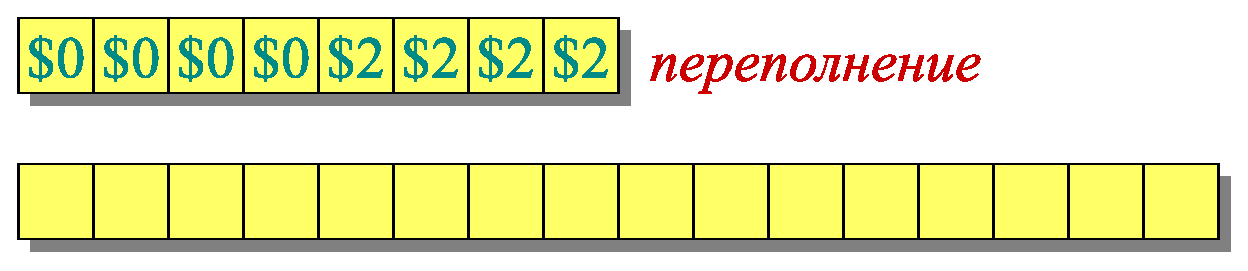
\includegraphics[width=3in]{lecture13/accountant1.eps}
  \caption{Состояния перед удваиванием таблицы}
  \label{fig:acc1}
\end{figure}

\begin{figure}[ht]
  \centering
  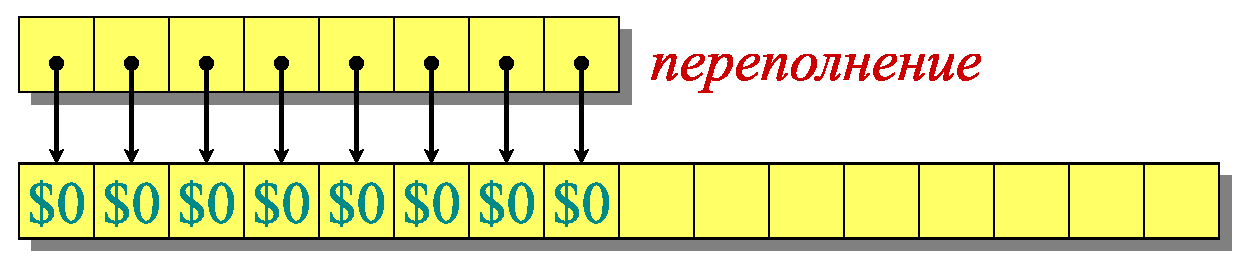
\includegraphics[width=3in]{lecture13/accountant2.eps}
  \caption{Копирование ячеек}
  \label{fig:acc2}
\end{figure}

\begin{figure}[ht]
  \centering
  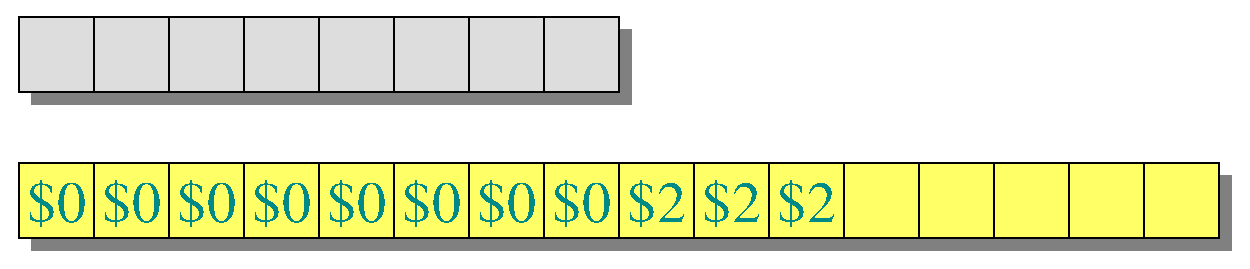
\includegraphics[width=3in]{lecture13/accountant3.eps}
  \caption{После удваивания таблицы}
  \label{fig:acc3}
\end{figure}

Добавим в нашу таблицу значения амортизированной стоимости:

\begin{center}
\begin{tabular}{|r|c|c|c|c|c|c|c|c|c|c|}
  \hline
      $i$ & 1 & 2 & 3 & 4 & 5 & 6 & 7 & 8 & 9  & 10 \\
  \hline
 $size_i$ & 1 & 2 & 4 & 4 & 8 & 8 & 8 & 8 & 16 & 16 \\
  \hline
    $c_i$ & 1 & 2 & 3 & 1 & 5 & 1 & 1 & 1 & 9  & 1 \\
  \hline
    $c_i$ & 1 & 1 & 1 & 1 & 1 & 1 & 1 & 1 & 1 & 1 \\
          & 0 & 1 & 2 & 0 & 4 & 0 & 0 & 0 & 8 & 1 \\
  \hline
$\hat{c}_i$ & $2^*$ & 3 & 3 & 3 & 3 & 3 & 3 & 3 & 3 & 3 \\
  \hline
   $bank_i$ & 1 & 2 & 2 & 4 & 2 & 4 & 6 & 8 & 2 & 4 \\  
  \hline
\end{tabular}
\end{center}

Соблюдается инвариант: баланс в банке никогда не меньше нуля, соответственно
амортизированные стоимости определяют верхнюю границу для фактических
стоимостей. Получаем границу в $\Theta(n)$.

\end{document}

